\section{Computer vision using neural networks}

Based on the comparison and elaboration presented previously, it was decided that a computer-vision based system would be necessary for the successful completion of the project. In particular, the object detector should,

\begin{itemize}
	\item Not require a beacon, light or any other object to be placed on the object,
	\item Locate the object with high accuracy,
	\item Be able to differentiate between classes of objects, while treating different instances of the same class equally (in other words, locate \emph{any} cheetah regardless of its specific spot pattern),
	\item Have a low enough latency that the object can't escape the field of view of the cameras before a result is reached,
	\item Work robustly - this means locating the regardless of its orientation, lighting, specific shape, background, and so on - and finally,
	\item Be able to track any other object with minimal extra work or design required, should the focus of research be changed.
\end{itemize}

This chapter details the literature surrounding the method which achieve these requirements. Since computer vision is an extremely large field of study on its own, the only concepts discussed are those which one must absolutely know for the completion of this project.

\subsection{Basic computer vision concepts}
Photo-based computer vision techniques tend to be able to differentiate between classes of objects by using a number of cascaded filters, with each layer of filters being able to detect more and more complex shapes in an image. These filters are known as 'kernels', and tend to be implemented as square matrices which are convolved with the input image, a 2D array of pixel values.

As an example, Figure~\ref{fig:input_output_simple_filter} shows a simple image before (left) and after (right) being convolved with a vertical line finding kernel.

\begin{figure}[h!]%
    \centering
    \subfloat{{
\includegraphics[width=3cm]{literature_review/input_image} }}%
    \qquad \qquad
    \subfloat{{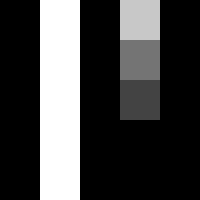
\includegraphics[width=3cm]{literature_review/output_image} }}%
    \caption{An image, before (left) and after (right) being convolved with a vertical line finder.}%
    \label{fig:input_output_simple_filter}%
\end{figure}

Note how the the vertical line in the left part of the input has been found (represented by bright pixels in the output image). The horizontal line on the bottom right has been rejected. The faint vertical line in the top right has been found, albeit faintly. The exact same transformation is shown below, where the images have been replaced with their underlying matrices. The leftmost matrix is the pixel values of the input matrix, the middle is the kernel and the rightmost matrix is the output. \\

\begin{table}[h!]
	\centering
	\begin{tabular}{ p{0.5cm} p{0.5cm} p{0.5cm} p{0.5cm} p{0.5cm} p{0.5cm} p{0.5cm} p{0.5cm} p{0.5cm} p{0.5cm} p{0.5cm} p{0.5cm} p{0.5cm} p{0.5cm} p{0.5cm}}
 5 & 232 & 180 & 212 & 180 &           &    &   &    &   & 0 & 255 & 0 & 200 & 0 \\
30 & 243 & 152 & 206 & 188 &           & -1 & 2 & -1 &   & 0 & 255 & 0 & 116 & 0 \\
32 & 255 & 210 & 190 & 190 & $\otimes$ & -1 & 2 & -1 & = & 0 & 255 & 67 & 0  & 0 \\
11 & 242 & 235 & 230 & 210 &           & -1 & 2 & -1 &   & 0 & 255 & 0 &  0  & 0 \\
90 & 240 & 130 &  20 &  30 &           &    &   &    &   & 0 & 255 & 0 &  0  & 0
	\end{tabular}
\end{table}

A larger, more interesting input image is shown below, in Figure~\ref{fig:image_kernel_demo}.

% TODO: reference http://setosa.io/ev/image-kernels/
\begin{figure}[h!]
  \centering
  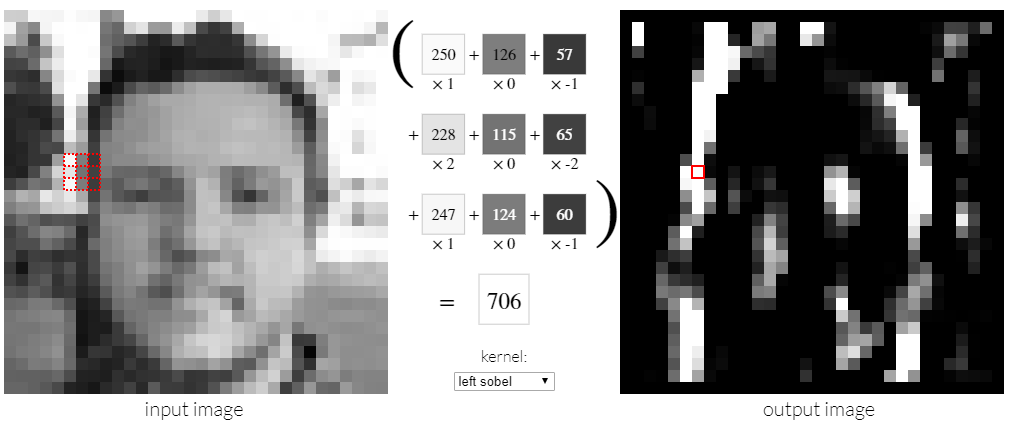
\includegraphics[width=\textwidth]{literature_review/image_kernel_demo}
  \caption{\label{fig:image_kernel_demo} A demonstration of image convolution on a photo of a human.}
\end{figure}

The output image on the right hand side is the result of applying an edge-emphasizing filter. Note how the vertical lines around the shape of the face and nose are highlighted.

As an example of a complete system, consider a network of filters in which the first layer of kernels may detect vertical lines, angled lines, dots, and so on. These detections are then used as input matrices to the next layer, which will convolve them with a set of kernels to produce more complex detections. For example, two horizontal lines and two vertical lines may indicate the presence of a square in an image. A different configuration of lines may indicate a circle, and so on.

Carefully designing and combining these filters can ultimately result in the detection of an object. However, this method is incredibly time consuming and requires extensive domain-specific knowledge. Even after the work has been put in to locate one type of object in a frame, locating another type of object may require the user to start from scratch.

\subsection{A brief introduction to machine learning}

Luckily, there exist other methods to find values for the kernels mentioned previously: instead of hand-selecting each kernel kernel value, one could instead use machine-learning techniques (in which computers use datasets data 'learn' the parameters of a model) to create kernels with 'optimal' values to find objects in a frame. This boils down to using data (known input-output pairs of an image of cheetah, and the label "cheetah") to optimize the kernel values in the network of filters.

The standard method of doing this for images is through the use of Convolutional Neural Networks (CNNs), a class of large artificial neural networks. They typically consist of layers of kernels (as discussed previously) along with an array of other operations borrowed from the fields of computer vision and machine learning.

{\color{red} talk a bit about neural networks (mainly fully connected layer type stuff) and include an image. mention the multi-layer perceptron. This part needs some work}

CNNs are initialized with random values in their kernels and random values for the transformations which combine the outputs of their kernels - only their general architecture tends to be fixed by human practitioners. These values are known as 'weights'. A summary of the method to get an optimal set of weights is as follows:
%These values are known in the field as 'weights', while calculations are performed by 'neurons' - nodes in the CNN which perform an operation.

\begin{enumerate}
\item Initialize the CNN with a set structure and random weights.
\item Pass an image through the CNN, and take note of the output.
\item Get the error (the difference between the CNN output and the correct answer) and propagate it back through the CNN, adjusting the weights \emph{slightly} in such a way that that same input would be more likely to produce the correct output if run again. This is known as 'back-propagation'.
\item Repeat the first three steps a few hundred or thousand times until the performance stops increasing. It is helpful to use a large dataset consisting of a diverse set of images.
\end{enumerate}

This process is known as 'training'.

While it is possible that the CNN will act as an inefficient look-up table (mapping those specific inputs to their correct outputs, but giving the wrong result for a new image which it hasn't been exposed to) it is hoped that the CNN will instead map any \emph{similar} input to the correct output. As an example, a correct training CNN will map any image which \emph{looks} like a cheetah (has the correct body structure, spots, ear location, etc) to an output which is numerically encoded to represent "cheetah". The process of taking an input and producing an output is known as 'inferencing'.

It should be noted that CNNs are nothing more than a mapping from a vector of input pixels (the image) to a vector which represents certain outputs (such as "cheetah", "no cheetah" or even the coordinates of a cheetah). Thus, in essence, this entire process is the solution to an optimisation problem: how to find the best set of weights to correctly map an input to the correct output.

CNNs simply require a few hundred or thousand labelled images and a few hours on a modern GPU. There are many tips, tricks and open datasets which can be used to make this work easier.

\subsection{Key machine learning concepts and definitions}
Before getting lost in activation functions, dropout and the rest of the endless list of ideas in machine learning, it is worth considering the separation of jobs in in modern data science. Typically, there is one team which designs the neural network architecture, tunes hyper-parameters (important parameters usually set by humans), publishes results, and so on. This requires a certain set of skills.

Next, another person with a separate skill set puts the neural network into production in order to achieve some goal - possibly after retraining it on some other dataset. If you find yourself in the second group of people, you don't tend to need to keep up with every new paper published. Instead, armed with some understanding of the main innovations in each network design, you only need compare some training techniques and architectures as a whole.

Since the project at hand doesn't necessitate a brand new architecture, we find ourselves firmly in the latter group. Thus, only a few ideas need to be discussed.

\subsubsection{General terminology}

\textit{Machine learning, neural networks, deep learning, CNNs}: machine learning is the branch of computer science involved in fitting a model using data alone. Neural networks are a subset of machine learning, specifying a class of architectures loosely inspired by the synapses in the nervous system of an organic brain. Deep learning is the relatively recent practice of creating especially long neural networks in order to represent more complex mappings. Finally, CNNs are a subset of deep learning, in which the synapses of a deep neural network are kernels which perform convolution operations.

\textit{Image classification vs object detection:} an image classifier indicates \emph{what} objects are in an image. An object detector finds what objects are in the image, and also \emph{where} in the image they can be found. One might think to perform object detection using an image classification CNN by dividing an input image into a grid of smaller overlapping images, and then passing these smaller images to the CNN. By noting which objects are detected in each image, one could estimate where in the original image the object can be found. Interestingly, this is almost exactly what object detectors do internally! In fact, ignoring some minor details like 'strides' and 'pooling', it's almost exactly what convolution with a kernel does. Newer object detection architectures are internally a lot more sophisticated than this but operate with the same intuition.

\textit{Bounding box:} also known as an anchor, a bounding box is a pair of points which determine a box around a detected object. Two $(x, y)$ pairs of numbers are usually part of the output of an object detection neural network.

{\Huge \color{red} show image from picam with things around objects}

\subsubsection{\color{red} Find a name for this}

\textit{Feature extractor:} it is common practice to concatenate an well-designed existing neural network architecture with another architecture to produce a new, larger model which performs an overall more complex task. Thus, the role of the first part of the new model is to extract useful features for the second part to process. In this way, neural networks can be a bit like Lego.

\textit{Transfer learning:} this refers to the practice in which the weights of one neural network are copied to another network. This enables problems to be solved using much less data than neural networks ordinarily require, as the weights are already quite good before the retraining process. The idea is that the early layers are likely to have been trained to find very general features in the image (such as lines, circles, eyes, tails, etc). These are often relevant to a wide variety of problems. This is why a trained network will often have its training dataset specified - the content of the training dataset is a good indicator of whether transfer learning would help in a different problem.

\subsubsection{Training-specific terminology}

\textit{Epoch:}

\textit{Batch size:}

\textit{Loss:}

\textit{Optimizers:}






\subsection{A brief introduction to neural accelerator sticks}
CNNs tend to require a large number of operations to produce an output. The exact amount of computation required depends on the neural network architecture, though even relatively small object detectors generally require on the order of millions of multiply-accumulate instructions with significant amounts of data being loaded to and from the various levels of cache. Combined with the slower processor on many mobile computer platforms, the neural network would not be able to run in real time. As an example of the inference times involved, a cutting edge object detection network designed for use on mobile devices typically requires around one full second to infer a result on the CPU of a Raspberry Pi model 3.

Fortunately, this work can be easily parallelized over multiple processing cores. To this end, there are three types of parallelization which tend to occur: during the application of kernels, during matrix multiplication and in parts of the neural network where the data flow is naturally parallel. This work is a perfect fit for GPUs, which contain a large number of processing cores designed for such tasks. However, since GPU support for CNNs on non-NVIDIA devices is lacking, other means had to be investigated.

% https://petewarden.com/2014/08/07/how-to-optimize-raspberry-pi-code-using-its-gpu/
% https://rpiplayground.wordpress.com/2014/05/03/hacking-the-gpu-for-fun-and-profit-pt-1/

\textit{For the rest of this chapter, assume any obscure words have been patented by Intel$^{^{\ TM}}$ or one of its subsidiaries.}

To solve this problem, some chip makers have started to produce 'neural accelerators' - devices which use parallelization to decrease the inference time of neural network. One such as the Movidius Neural Compute Stick (NCS), a specialized neural network accelerator which plugs into an underpowered device (such a Raspberry Pi) to offload and speed up inferencing time. Its purpose-built processing cores typically result in inference speed increases of between $700\%$ and $1000\%$. This is the benefit of being purpose built for CNNs.

The operation of the Movidius NCS is as follows: first, the user designs and trains their neural network. Next, they compile it down to a specific format optimized for the NCS and upload it to the device. From then on, the user can send preprocessed images to the NCS, wait for the inference to occur, and then retrieve the result.

The actual processing is done using Intel's Myriad 2 Vision Processing Unit (VPU), which makes use of 12 specially designed processing cores named 'shaves'.

%\begin{figure}[h!]
%  \centering
%  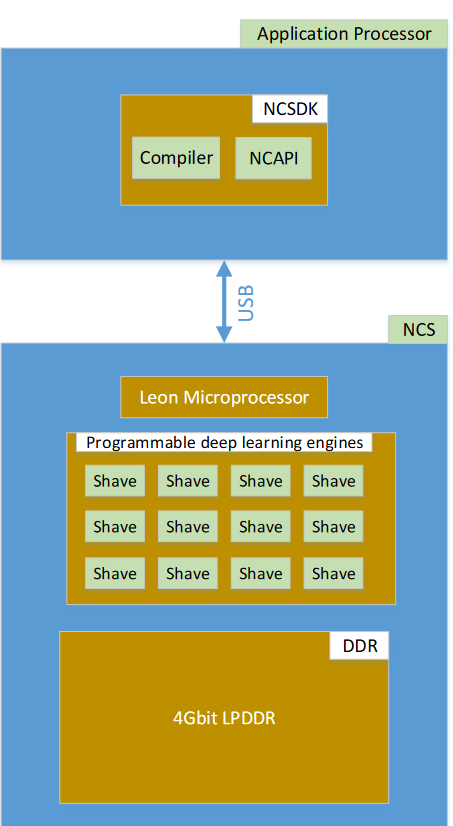
\includegraphics[width=0.4\textwidth]{literature_review/NCS_internals}
%  \caption{\label{fig:NCS_internals} Internals of the Movidius Neural Compute Stick.}
%\end{figure}


\subsection{Comparison of neural network architectures}
Not all neural network architectures are equal. Differences between models generally include,

\begin{itemize}
	\item Classification accuracy,
	\item Inference speed, which is a function of
	\begin{itemize}
		\item The number of operations (processing) and
		\item The number of weights (data retrieval)
	\end{itemize}
	\item The amount of data required for training/fine tuning,
	\item The existence (or lack) of pretrained models in each specific deep learning framework,
	\item Whether recent innovations in the field have been included, and
	\item The underlying method in which objects are detected and localised within the image
\end{itemize}

{\Huge \color{red} how should i finish this off? ack!}

%Newer neural networks often take ideas from older architectures. Sometimes, they even include all or most of a previous architecture as part of the design of the new model. An example of this is MobileNet - an architecture designed at Google, aimed to run quickly on modern mobile devices (such as newer smartphones). A common practice is to train MobileNet to classify objects on a given dataset, then remove the final layers, concatenate it with another model (with MobileNet acting as a feature extractor) and end up with an object detector.

%Since MobileNet was designed for mobile devices, it traded some classification accuracy for performance. However, the architecture is remarkable in that the performance increase is significant while the classification accuracy decrease is not.

%Next was the choice of the actual object detector. There are two (TODO: check this) main ideas for this approach: one could get an image classifier and apply it to the image multiple times (such as 25 times) resulting in a grid of overlapping detections.
